\documentclass[a4paper,12pt]{article}

\usepackage{float}


\usepackage[utf8]{inputenc}
\usepackage[dvips]{graphicx}
%\usepackage{a4wide}
\usepackage{epsfig}
\usepackage{fancybox}
\usepackage{verbatim}
\usepackage{array}
\usepackage{latexsym}
\usepackage{alltt}
\usepackage{amssymb}
\usepackage{amsmath,amsthm}
\usepackage{bm}
\usepackage{wasysym}

%\usepackage{fullpage}
%\usepackage{hyperref}
\usepackage{listings}
\usepackage{color}
\usepackage{algorithm}
\usepackage{algpseudocode}
\usepackage[hmargin=2cm,vmargin=3.0cm]{geometry}
%\topmargin=0cm
%\topmargin=-1.8cm
%\addtolength{\textheight}{6.5cm}
%\addtolength{\textwidth}{2.0cm}
%\setlength{\leftmargin}{-3cm}
%\setlength{\oddsidemargin}{0.0cm}
%\setlength{\evensidemargin}{0.0cm}

%misc libraries goes here
\usepackage{tikz}
\usepackage{tikz-qtree}
\usetikzlibrary{automata,positioning}

\usepackage{multicol}
\usepackage{enumitem}

\usepackage[most]{tcolorbox}

\usepackage[colorlinks=true,urlcolor=black,linkcolor=black]{hyperref}


\lstdefinestyle{customtex}{
    %backgroundcolor=\color{lbcolor},
    tabsize=2,
    language=TeX,
    numbers=none,
    basicstyle=\footnotesize\ttfamily,
    numberstyle=\footnotesize,
    aboveskip={0.0\baselineskip},
    belowskip={0.0\baselineskip},
    %
    columns=flexible,
    keepspaces=true,
    fontadjust=true,
    upquote=true,
    %
    breaklines=true,
    prebreak=\raisebox{0ex}[0ex][0ex]{\ensuremath{\hookleftarrow}},
    frame=single,
    showtabs=false,
    showspaces=false,
    showstringspaces=false,
    %
    %identifierstyle=\color[rgb]{0,0.2,0.8},
    identifierstyle=\color[rgb]{0,0,0.5},
    %identifierstyle=\color[rgb]{0.133,0.545,0.133},
    %keywordstyle=\color[rgb]{0.8,0,0},
    %keywordstyle=\color[rgb]{0.133,0.545,0.133},
    keywordstyle=\color[rgb]{0,0,0.5},
    %commentstyle=\color[rgb]{0.133,0.545,0.133},
    commentstyle=\color[rgb]{0.545,0.545,0.545},
    %stringstyle=\color[rgb]{0.827,0.627,0.133},
    stringstyle=\color[rgb]{0.133,0.545,0.133},
    %
    literate={â}{{\^{a}}}1 {Â}{{\^{A}}}1 {ç}{{\c{c}}}1 {Ç}{{\c{C}}}1 {ğ}{{\u{g}}}1 {Ğ}{{\u{G}}}1 {ı}{{\i}}1 {İ}{{\.{I}}}1   {ö}{{\"o}}1 {Ö}{{\"O}}1 {ş}{{\c{s}}}1 {Ş}{{\c{S}}}1 {ü}{{\"u}}1 {Ü}{{\"U}}1 {~}{$\sim$}{1}
}

\lstdefinestyle{output}{
    %backgroundcolor=\color{lbcolor},
    tabsize=2,
    numbers=none,
    basicstyle=\footnotesize\ttfamily,
    numberstyle=\footnotesize,
    aboveskip={0.0\baselineskip},
    belowskip={0.0\baselineskip},
    %
    columns=flexible,
    keepspaces=true,
    fontadjust=true,
    upquote=true,
    %
    breaklines=true,
    prebreak=\raisebox{0ex}[0ex][0ex]{\ensuremath{\hookleftarrow}},
    frame=single,
    showtabs=false,
    showspaces=false,
    showstringspaces=false,
    %
    %identifierstyle=\color[rgb]{0.44,0.12,0.1},
    identifierstyle=\color[rgb]{0,0,0},
    keywordstyle=\color[rgb]{0,0,0},
    commentstyle=\color[rgb]{0,0,0},
    stringstyle=\color[rgb]{0,0,0},
    %
    literate={â}{{\^{a}}}1 {Â}{{\^{A}}}1 {ç}{{\c{c}}}1 {Ç}{{\c{C}}}1 {ğ}{{\u{g}}}1 {Ğ}{{\u{G}}}1 {ı}{{\i}}1 {İ}{{\.{I}}}1   {ö}{{\"o}}1 {Ö}{{\"O}}1 {ş}{{\c{s}}}1 {Ş}{{\c{S}}}1 {ü}{{\"u}}1 {Ü}{{\"U}}1
}

\lstset{style=customtex}


\tikzset{%
    terminal/.style={draw, rectangle,
    				 align=center, 
					 minimum height=1cm, 
					 minimum width=2cm,
					 fill=black!10,
					 anchor=mid},
    nonterminal/.style={draw, rectangle,
    					align=left,
					    minimum height=1cm, 
						minimum width=2cm, 
						anchor=mid},% and so on
}

%% Style for terminals
%\tikzstyle{terminal}=[draw, rectangle, 
%					  minimum height=1cm, 
%					  minimum width=2cm, 
%					  fill=black!20,
%					  anchor=south west]
%% Style for nonterminals
%\tikzstyle{nonterminal}=[draw, rectangle, 
%						 minimum height=1 cm, 
%						 minimum width=2 cm, 
%						 anchor=north east]


\newcommand{\HRule}{\rule{\linewidth}{1mm}}
\newcommand{\kutu}[2]{\framebox[#1mm]{\rule[-2mm]{0mm}{#2mm}}}
\newcommand{\gap}{ \\[1mm] }

\newcommand{\Q}{\raisebox{1.7pt}{$\scriptstyle\bigcirc$}}
\newcommand{\minus}{\scalebox{0.35}[1.0]{$-$}}

\setlength{\fboxsep}{10pt}

\tcbsetforeverylayer{enhanced jigsaw, breakable, arc=0mm, boxrule=1pt, boxsep=5pt, after=\vspace{1em}, colback=white, colframe=black}

\newcolumntype{P}[1]{>{\centering\arraybackslash}p{#1}}

\setlength\parindent{0pt}

%\renewcommand\arraystretch{1.2}

\newenvironment{Tab}[1]
  {\def\arraystretch{1}\tabular{#1}}
  {\endtabular}

%%%%%%%%%%%%%%%%%%%%%%%%%%%%%%%%%%%%%%%%%%%%%%%%%%%%%%%%%%%%%%%%%%%%%%%%%%%%%%%%%%%%%%

\title{Formal Languages and Abstract Machines \\ Take Home Exam 2}
\author{Beyazıt Yalçınkaya \\ 2172138} % write your name and id
\date{} % do not write any date

%%%%%%%%%%%%%%%%%%%%%%%%%%%%%%%%%%%%%%%%%%%%%%%%%%%%%%%%%%%%%%%%%%%%%%%%%%%%%%%%%%%%%%

\begin{document}
\HRule\\
Middle East Technical University \hfill Department of Computer Engineering
{\let\newpage\relax\maketitle}
\HRule\\
\vspace{1cm}

%%%%%%%%%%%%%%%%%%%%%%%%%%%%%%%%%%%%%%%%%%%%%%%%%%%%%%%%%%%%%%%%%%%%%%%%%%%%%%%%%%%%%%

% Write your answers below the section tags
\section{Context-Free Grammars \hfill \normalfont{(10 pts)}}

\paragraph{a)} Give the rules of the Context-Free Grammars to recognize strings in the given languages where $\Sigma=\{a,b\}$ and $S$ is the start symbol. \\  

$L(G)=\{w \mid \;  w \in \Sigma^*;\; |w| \geq 3;\; $  \hfill \small{(2/10 pts)} \\
\hspace*{22mm} the first and the second from the last symbols of $w$ are the same$\}$ \\

\begin{tcolorbox}
$
S \rightarrow aTaa \mid aTab \mid bTbb \mid bTba \\
T \rightarrow aT \mid bT \mid \varepsilon
$
\end{tcolorbox}


$L(G)=\{w \mid \;  w \in \Sigma^*;\; $ the length of w is odd$\}$ \hfill \small{(2/10 pts)} \\

\begin{tcolorbox}
$
S \rightarrow aSa \mid aSb \mid bSa \mid bSb \mid a \mid b
$
\end{tcolorbox}


$L(G)=\{w \mid \;  w \in \Sigma^*;\; n(w,a)=2\cdot n(w,b)\}$ where $n(w,x)$ is the number of $x$ symbols in $w$ \hfill \small{(3/10 pts)} \\

\begin{tcolorbox}
$
S \rightarrow TaTaTbT \mid TaTbTaT \mid TbTaTaT \\
T \rightarrow TaTaTbT \mid TaTbTaT \mid TbTaTaT \mid \varepsilon
$
\end{tcolorbox}



\paragraph{b)} Find the set of strings recognized by the CFG rules given below:         \hfill \small{(3/10 pts)} \\


$S \to X \mid Y$ \\
$X \to aXb \mid A \mid B$ \\
$A \to aA \mid a$ \\
$B \to Bb \mid b$ \\
$Y \to CbaC$ \\
$C \to CC \mid a \mid b \mid \varepsilon$  \\

\begin{tcolorbox}
$
L = \{a^nb^m \mid n \neq m, \ n, m \geq 1, \ n, m \in \mathbb{N}^+\} \cup \{w \in \{a, b\}^* \mid w \text{ contains }ba\}
$
\end{tcolorbox}


\newpage
\section{Parse Trees and Derivations \hfill \normalfont{(20 pts)}}
Given the CFG below, provide parse trees for given sentences in \textbf{a} and \textbf{b}.\\

\begin{lstlisting}[style=output,mathescape=true]
S   $\to$ NP VP
VP  $\to$ V NP | V NP PP
PP  $\to$ P NP
NP  $\to$ N | D N | NP PP
V   $\to$ wrote | built | constructed
D   $\to$ a | an | the | my
N   $\to$ John | Mary | Jane | man | book | automata | pen | class
P   $\to$ in | on | by | with
\end{lstlisting}

\paragraph{a)} Jane constructed automata with a pen \hfill \small{(4/20 pts)} \\

\begin{tcolorbox}
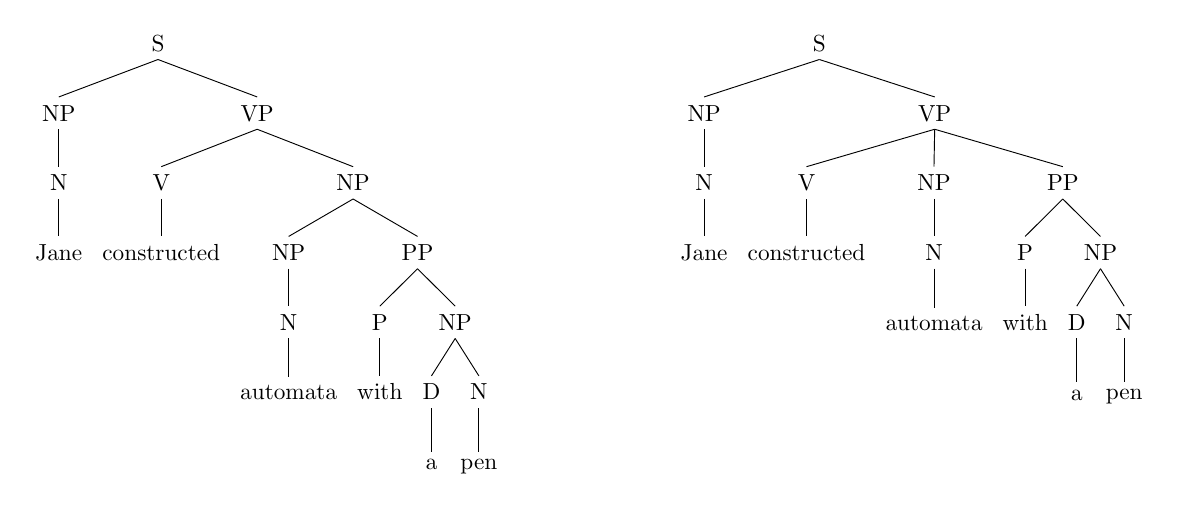
\begin{tikzpicture}[scale = 0.84]
\Tree [.S [.NP [.N Jane ] ] [.VP [.V constructed ] [.NP [.NP [.N automata ] ] [.PP [.P with ] [.NP [.D a ] [.N pen ] ] ] ] ] ]
\begin{scope}[xshift = 10 cm]
\Tree [.S [.NP [.N Jane ] ] [.VP [.V constructed ] [.NP [.N automata ] ] [.PP [.P with ] [.NP [.D a ] [.N pen ] ] ] ] ]
\end{scope}
\end{tikzpicture}
\end{tcolorbox}

\paragraph{b)} my book in the man built a Jane by a pen \hfill \small{(4/20 pts)} \\

\begin{tcolorbox}
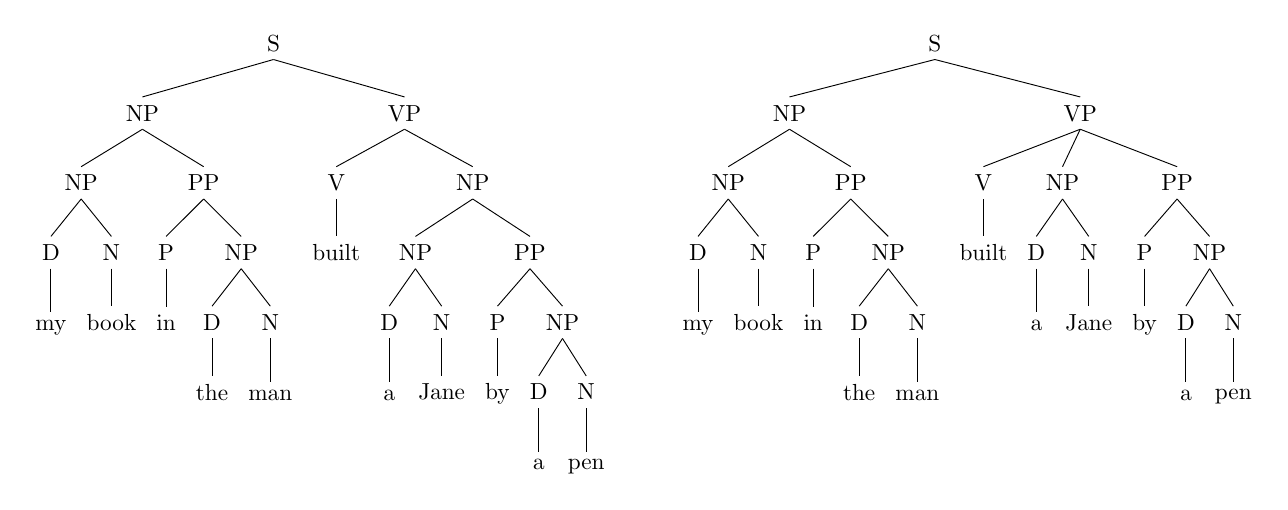
\begin{tikzpicture}[scale = 0.84]
\Tree [.S [.NP [.NP [.D my ] [.N book ] ] [.PP [.P in ] [.NP [.D the ] [.N man ] ] ] ] [.VP [.V built ] [.NP [.NP [.D a ] [.N Jane ] ] [.PP [.P by ] [.NP [.D a ] [.N pen ] ] ] ] ] ]
\begin{scope}[xshift = 10 cm]
\Tree [.S [.NP [.NP [.D my ] [.N book ] ] [.PP [.P in ] [.NP [.D the ] [.N man ] ] ] ] [.VP [.V built ] [.NP [.D a ] [.N Jane ] ] [.PP [.P by ] [.NP [.D a ] [.N pen ] ] ] ] ]
\end{scope}
\end{tikzpicture}
\end{tcolorbox}

\newpage

Given the CFG below, answer \textbf{c}, \textbf{d} and \textbf{e} \\

\begin{lstlisting}[style=output,mathescape=true]
S  $\to$ E
E  $\to$ E + T | E - T | T
T  $\to$ T * I | T / I | I
I  $\to$ 0 | 1 | 2 | 3 | 4 | 6 | 7 | 8 | 9
\end{lstlisting}

\paragraph{c)} Provide the left-most derivation of 7 - 4 * 3 step-by-step and plot the final parse \hfill \small{(4/20 pts)} \\
tree matching that derivation \\

\begin{tcolorbox}
$
D_L = 
S \Rightarrow
E \Rightarrow
E - T \Rightarrow
T - T \Rightarrow
I - T \Rightarrow
7 - T \Rightarrow
7 - T * I \Rightarrow
7 - I * I \Rightarrow
7 - 4 * I \Rightarrow
7 - 4 * 3
$
\begin{center}
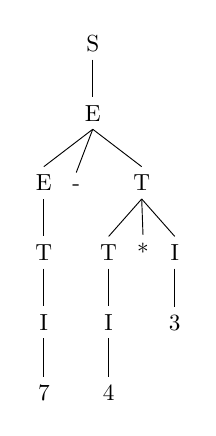
\begin{tikzpicture}[scale = 0.84]
\Tree [.S [.E [.E [.T [.I 7 ] ] ] - [.T [.T [.I 4 ] ] * [.I 3 ] ] ] ]
\end{tikzpicture}
\end{center}
\end{tcolorbox}

\paragraph{d)} Provide the right-most derivation of 7 - 4 * 3 step-by-step and plot the final parse \hfill \small{(4/20 pts)} \\
 tree matching that derivation \\
 
\begin{tcolorbox}
$
D_R = 
S \Rightarrow
E \Rightarrow
E - T \Rightarrow
E - T * I \Rightarrow
E - T * 3 \Rightarrow
E - I * 3 \Rightarrow
E - 4 * 3 \Rightarrow
T - 4 * 3 \Rightarrow
I - 4 * 3 \Rightarrow
7 - 4 * 3
$
\begin{center}
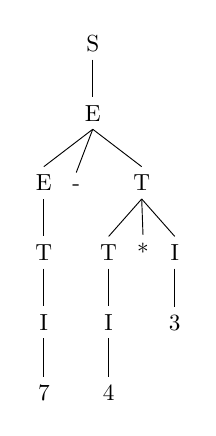
\begin{tikzpicture}[scale = 0.84]
\Tree [.S [.E [.E [.T [.I 7 ] ] ] - [.T [.T [.I 4 ] ] * [.I 3 ] ] ] ]
\end{tikzpicture}
\end{center}
\end{tcolorbox}


\paragraph{e)} Are the derivations in \textbf{c} and \textbf{d} in the same similarity class?  \hfill \small{(4/20 pts)} \\

\begin{tcolorbox}
Yes, since $(D_L, D_R)$ belongs in the reflexive, symmetric, transitive closure of $\prec$.
\end{tcolorbox}


\newpage
\section{Pushdown Automata \hfill \normalfont{(30 pts)}}

\paragraph{a)} 
Find the language recognized by the PDA given below \hfill \small{(5/30 pts)} \\

\begin{tikzpicture}[shorten >=1pt,node distance=3cm,on grid,auto]
\node[state,initial,initial text=] (q_0) {$q_0$};
\node[state] (q_1) [right=of q_0] {$q_1$};
\node[state] (q_2) [above right=of q_1] {$q_2$};
\node[state] (q_3) [below right=of q_1] {$q_3$};
\node[state,accepting](q_4) [right=of q_2] {$q_4$};
\node[state](q_5) [right=of q_3] {$q_5$};
\node[state,accepting](q_6) [right=of q_5] {$q_6$};
\path[->]

(q_0) edge node {$\varepsilon,\varepsilon \to \#$} (q_1)
(q_1) edge [loop below] node {$x,\varepsilon \to x$} (q_1)

%%
(q_1) edge node {$\varepsilon,\varepsilon \to \varepsilon$} (q_2)
(q_2) edge [loop above] node {$y,x \to \varepsilon$} (q_2)

(q_2) edge node {$\varepsilon,\# \to \varepsilon$} (q_4)
(q_4) edge [loop above] node {$z,\varepsilon \to \varepsilon$} (q_4)

%%%

(q_1) edge node {$\varepsilon,\varepsilon \to \varepsilon$} (q_3)
(q_3) edge [loop below] node {$y,\varepsilon \to \varepsilon$} (q_3)

(q_3) edge node {$\varepsilon,\varepsilon \to \varepsilon$} (q_5)
(q_5) edge [loop below] node {$z,x \to \varepsilon$} (q_5)

(q_5) edge node {$\varepsilon,\# \to \varepsilon$} (q_6)
;
\end{tikzpicture} \\

\begin{minipage}{0.60\textwidth}
where the transition $((q_i,\alpha,\beta),(q_j,\gamma)) $ is represented as: 
\end{minipage}
\begin{minipage}{0.30\textwidth}
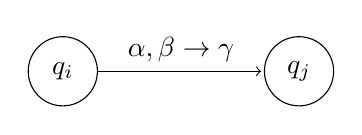
\begin{tikzpicture}[shorten >=1pt,node distance=3cm,on grid,auto]
\node[state] (q_i) {$q_i$};
\node[state] (q_j) [right=of q_i] {$q_j$};
\path[->]
(q_i) edge node {$\alpha,\beta \to \gamma$} (q_j);
\end{tikzpicture} \\
\end{minipage}


\begin{tcolorbox}
$
L = \{x^ny^nz^m \mid n, m \geq 0, \ n, m \in \mathbb{N}\} \cup \{x^ny^mz^n \mid n, m \geq 0, \ n, m \in \mathbb{N}\}
$
\end{tcolorbox}


\paragraph{b)} 
Design a PDA to recognize language $ L=\{x^n y^{m+n} x^m \mid \; n,m \geq 0; \; n,m \in \mathbb{N}  \} $  \hfill \small{(5/30 pts)} \\

\begin{tcolorbox}
\begin{center}
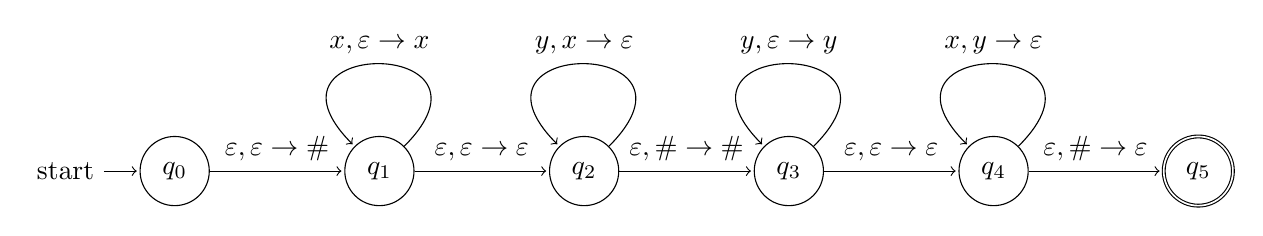
\begin{tikzpicture}[shorten >=1 pt, node distance = 2.6 cm, on
grid, auto]
\node [state, initial] (q_0) {$q_0$};
\node [state] (q_1) [right = of q_0] {$q_1$};
\node [state] (q_2) [right = of q_1] {$q_2$};
\node [state] (q_3) [right = of q_2] {$q_3$};
\node [state] (q_4) [right = of q_3] {$q_4$};
\node [state, accepting] (q_5) [right = of q_4] {$q_5$};
\path [->]
(q_0)edge node {$\varepsilon, \varepsilon \rightarrow \#$} (q_1)
(q_1)edge node {$\varepsilon, \varepsilon \rightarrow \varepsilon$} (q_2) edge [loop] node [above] {$x, \varepsilon \rightarrow x$} (q_1)
(q_2)edge node {$\varepsilon, \# \rightarrow \#$} (q_3) edge [loop] node [above] {$y, x \rightarrow \varepsilon$} (q_2)
(q_3)edge node {$\varepsilon, \varepsilon \rightarrow \varepsilon$} (q_4) edge [loop] node [above] {$y, \varepsilon \rightarrow y$} (q_3)
(q_4)edge node {$\varepsilon, \# \rightarrow \varepsilon$} (q_5) edge [loop] node [above] {$x, y \rightarrow \varepsilon$} (q_4);
\end{tikzpicture}
\end{center}
\end{tcolorbox}

\newpage

\paragraph{c)} 
Design a PDA to recognize language $ L=\{x^n y^m \mid \; n < m \leq 2n; \; n,m \in \mathbb{N^+} \} $  \hfill \small{(10/30 pts)} \\
Do not use multi-symbol push/pop operations in your transitions. \\
Simulate the PDA on strings \textit{xxy} (with only one rejecting derivation) and \textit{xxyyyy} (accepting derivation) with transition tables. \\


\begin{tcolorbox}
\begin{center}
\begin{tikzpicture}[shorten >=1 pt, node distance = 3 cm, on
grid, auto]
\node [state, initial] (q_0) {$q_0$};
\node [state] (q_1) [right = of q_0] {$q_1$};
\node [state] (q_2) [above = of q_1] {$q_2$};
\node [state] (q_3) [right = of q_1] {$q_3$};
\node [state] (q_4) [below = of q_3] {$q_4$};
\node [state] (q_5) [right = of q_3] {$q_5$};
\node [state, accepting] (q_6) [right = of q_5] {$q_6$};
\path [->]
(q_0) edge node {$\varepsilon, \varepsilon \rightarrow \#$} (q_1)
(q_1) edge [bend right] node [right] {$x, \varepsilon \rightarrow x$} (q_2)
edge node {$\varepsilon, x \rightarrow x$} (q_3)
(q_2)edge [bend right] node [left] {$\varepsilon, \varepsilon \rightarrow x$} (q_1)
(q_3)edge [loop] node [above] {$x, \varepsilon \rightarrow x$} (q_3)
edge [bend right] node [left] {$x, \varepsilon \rightarrow x$} (q_4)
edge node {$\varepsilon, \varepsilon \rightarrow \varepsilon$} (q_5)
(q_4)edge [bend right] node [right] {$\varepsilon, \varepsilon \rightarrow x$} (q_3)



(q_5) edge [loop] node [above] {$y, x \rightarrow \varepsilon$} (q_5)
edge node {$\varepsilon, \# \rightarrow \varepsilon$} (q_6);
\end{tikzpicture}
\end{center}

Table for $xxy$,
\begin{center}
\begin{tabular}{c | r | r | c}
	State & Unread Input & Stack & Transition Used \\ \hline
	$q_0$ & $xxy$ & $\varepsilon$ & $-$ \\
	$q_1$ & $xxy$ & $\#$ & $((q_0, \varepsilon, \varepsilon), (q_1, \#))$ \\
	$q_2$ & $xy$ & $x\#$ & $((q_1, x, \varepsilon), (q_2, x))$ \\
	$q_1$ & $xy$ & $xx\#$ & $((q_2, \varepsilon, \varepsilon), (q_1, x))$ \\
	$q_3$ & $xy$ & $xx\#$ & $((q_1, \varepsilon, x), (q_3, x))$ \\
	$q_3$ & $y$ & $xxx\#$ & $((q_3, x, \varepsilon), (q_3, x))$ \\
	$q_5$ & $y$ & $xxx\#$ & $((q_3, \varepsilon, \varepsilon), (q_5, \varepsilon))$ \\
	$q_5$ & $\varepsilon$ & $xx\#$ & $((q_5, y, x), (q_5, \varepsilon))$ \\
\end{tabular}
\end{center}

Table for $xxyyyy$,
\begin{center}
\begin{tabular}{c | r | r | c}
	State & Unread Input & Stack & Transition Used \\ \hline
	$q_0$ & $xxyyyy$ & $\varepsilon$ & $-$ \\
	$q_1$ & $xxyyyy$ & $\#$ & $((q_0, \varepsilon, \varepsilon), (q_1, \#))$ \\
	$q_2$ & $xyyyy$ & $x\#$ & $((q_1, x, \varepsilon), (q_2, x))$ \\
	$q_1$ & $xyyyy$ & $xx\#$ & $((q_2, \varepsilon, \varepsilon), (q_1, x))$ \\
	$q_3$ & $xyyyy$ & $xx\#$ & $((q_1, \varepsilon, x), (q_3, x))$ \\
	$q_4$ & $yyyy$ & $xxx\#$ & $((q_3, x, \varepsilon), (q_4, x))$ \\
	$q_3$ & $yyyy$ & $xxxx\#$ & $((q_4, \varepsilon, \varepsilon), (q_3, x))$ \\
	$q_5$ & $yyyy$ & $xxxx\#$ & $((q_3, \varepsilon, \varepsilon), (q_5, \varepsilon))$ \\
	$q_5$ & $yyy$ & $xxx\#$ & $((q_5, y, x), (q_5, \varepsilon))$ \\
	$q_5$ & $yy$ & $xx\#$ & $((q_5, y, x), (q_5, \varepsilon))$ \\
	$q_5$ & $y$ & $x\#$ & $((q_5, y, x), (q_5, \varepsilon))$ \\
	$q_5$ & $\varepsilon$ & $\#$ & $((q_5, y, x), (q_5, \varepsilon))$ \\
	$q_6$ & $\varepsilon$ & $\varepsilon$ & $((q_5, \varepsilon, \#), (q_6, \varepsilon))$ \\
\end{tabular}
\end{center}
\end{tcolorbox}

\newpage

\paragraph{d)} Given two languages $L'$ and $L$ as $L'=\{w \mid \; w\in L; \; |w|=4n+2 \; for\; n\in \mathbb{N} \}$
\hfill \small{(10/30 pts)} \\
If $L$ is a CFL, show that $L'$ is also a CFL by constructing an automaton for $L'$ in terms of another automaton that recognizes $L$. \\


\begin{tcolorbox}
Say alphabet of the language $L$ is $\Sigma$ and $L'' = \{w \in \Sigma^* \mid |w| = 4n + 2 \text{ for } n \in \mathbb{N}\}$. Then the language $L'$ can be interpreted as $L' = L \cap L''$. Note that $L''$ is a regular language so by the Theorem 3.5.2 (Elements of Theory of Computation, p.144), we know that $L'$ is a CFL. Now, we will formally construct an automaton for $L'$ to prove that it is, indeed, a CFL. Name the PDA that recognizes $L$ as $M_1 = (K_1, \Sigma, \Gamma_1, \Delta_1, s_1, F_1)$ and the DFA that recognizes $L''$ as $M_2 = (K_2, \Sigma, \delta, s_2, F_2)$. The PDA that recognizes $L'$ is defined $M = (K, \Sigma, \Gamma, \Delta, s, F)$ where,
\begin{itemize}
	\item $K = K_1 \times K_2$,
	\item $\Gamma = \Gamma_1$,
	\item $s = (s_1, s_2)$,
	\item $F = F_1 \times F_2$, and
	\item $\Delta$ is defined as follows, for each $((q_1, a, \beta), (q_1', \gamma)) \in \Delta_1$ and for each $q_2 \in K_2$, add $(((q_1, q_2), a, \beta), ((q_1', \delta(q_2, a)), \gamma))$ to $\Delta$ and  for each $((q_1, e, \beta), (q_1', \gamma)) \in \Delta_1$ and for each $q_2 \in K_2$, add $(((q_1, q_2), e, \beta), ((q_1', q_2), \gamma))$ to $\Delta$.
\end{itemize}
\end{tcolorbox}






\newpage
\section{Closure Properties \hfill \normalfont{(20 pts)}}

Let $L_1$ and $L_2$ be context-free languages which are not regular, and let $L_3$ be a regular language. Determine whether the following languages are necessarily CFLs or not. If they need to be context-free, explain your reasoning. If not, give one example where the language is a CFL and a counter example where the language is not a CFL. \\

\paragraph{a)} $L_4 = L_1 \cap (L_2 \setminus L_3)$ \hfill \small{(10/20 pts)} \\

\begin{tcolorbox}
Example for $L_4$ is not a CFL,\\
$
L_1 = \{a^nb^nc^m \mid n, m \geq 0, \ n, m \in \mathbb{N}\} \\
L_2 = \{a^nb^mc^m \mid n, m \geq 0, \ n, m \in \mathbb{N}\} \\
L_3 = \{\} \\
L_4 = L_1 \cap (L_2 \setminus L_3) = \{a^nb^nc^n \mid n \geq 0, \ n \in \mathbb{N}\}
$
\\\\
Example for $L_4$ is a CFL,\\
$
L_1 = \{a^nb^nc^m \mid n, m \geq 0, \ n, m \in \mathbb{N}\} \\
L_2 = \{a^nb^n \mid n \geq 0, \ n \in \mathbb{N}\} \\
L_3 = \{\} \\
L_4 = L_1 \cap (L_2 \setminus L_3) = \{a^nb^n \mid n \geq 0, \ n \in \mathbb{N}\}
$
\end{tcolorbox}

\paragraph{b)} $L_5 = (L_1 \cap L_3)\text{*}$ \hfill \small{(10/20 pts)} \\

\begin{tcolorbox}
By the Theorem 3.5.2 (Elements of Theory of Computation, p.144), the intersection of a CFL and a regular language is a CFL. Thus, $L_1 \cap L_3$ is a CFL. By the Theorem 3.5.1 (Elements of Theory of Computation, p.143), the CFLs are closed under union, concatenation, and Kleene star. Hence, $L_5$ is a CFL.
\end{tcolorbox}





\newpage
\section{Pumping Theorem \hfill \normalfont{(20 pts)}}

\paragraph{a)} Show that $L=\{a^n m^n t^i \mid \; n\leq i \leq 2n\}$ is not a Context Free Language \hfill \small{(10/20 pts)} \\
using Pumping Theorem for CFLs. \\

\begin{tcolorbox}
Assume that $L$ is a CFL and let $K$ be the pumping length. Then, by the Pumping Theorem, for the string $w = a^Km^Kt^K \in L$ there must be a split $uvxyz$ such that $|vy| \geq 1$, $|vxy| \leq K$, and $uv^ixy^iz \in L$ for every $i \geq 0$. There are five cases to consider, listed as follows,
\begin{enumerate}
	\item $vxy = a^j$ for some $1 \leq j \leq K$. $vy$ consists of $a$ symbols, pumping $i$ any value other than $i = 1$ would result into a string that is not in $L$, since number of $a$ symbols will be different than $K$ whereas number of $m$ symbols will stay as $K$.
	\item $vxy = m^j$ for some $1 \leq j \leq K$. $vy$ consists of $m$ symbols, pumping $i$ any value other than $i = 1$ would result into a string that is not in $L$, since number of $m$ symbols will be different than $K$ whereas number of $a$ symbols will stay as $K$.
	\item $vxy = t^j$ for some $1 \leq j \leq K$. $vy$ consists of $t$ symbols, pumping $i$ to $i = 3K$ would result into a string that is not in $L$. Since $vy$ contains at least $1$ and at most $K$ $t$ symbols, after pumping $w$ with $i = 3K$, number of $t$ symbols would be at least $3K > 2K$ and at most $4K - 1 > 2K$ which results into a string that is not in $L$.
	\item $vxy = a^jm^p$ for some $1 \leq j + p \leq K$. $vy$ consists of $a$ and $m$ symbols. Firstly, consider the case that $v$ contains $a$ symbols and $y$ contains $m$ symbols. In this case if $|v| = |y|$, then after pumping $i$ to $i = 2K$, the string will become at least $a^{2K}m^{2K}t^K$ and at most $a^{3K - 1}m^{3K - 1}t^K$ which is not in $L$. If $|v| \neq |y|$, then after pumping $i$ any value other than $i = 1$ would result into a string that has unequal number of $a$ and $m$ symbols which is not in $L$. Secondly, consider either $v$ contains both $a$ and $m$ symbols or $y$ contains both $a$ and $m$ symbols, then in this case pumping $i$ any value other than $i = 1$ would break the order of symbols in the string and result into a string that is not in $L$.
	\item $vxy = m^jt^p$ for some $1 \leq j + p \leq K$. $vy$ consists of $m$ and $t$ symbols. Firstly, consider the case that $v$ contains $m$ symbols and $y$ contains $t$ symbols. In this case pumping $i$ any value other than $i = 1$ would result into a string that has unequal number of $a$ and $m$ symbols which is not in $L$. Secondly, consider either $v$ contains both $m$ and $t$ symbols or $y$ contains both $m$ and $t$ symbols, then in this case pumping $i$ any value other than $i = 1$ would break the order of symbols in the string and result into a string that is not in $L$.
\end{enumerate}
Hence, in all cases it has been shown that pumping $i$ results into a string that is not in the language, this contradicts with the assumption. Assumption is discharged, $L$ is not a CFL.
\end{tcolorbox}

\newpage

\paragraph{b)} Show that $L=\{a^n b^{2n} a^n \mid \; n \in \mathbb{N+} \}$ is not a Context Free Language \hfill \small{(10/20 pts)} \\
using Pumping Theorem for CFLs. \\

\begin{tcolorbox}
Assume that $L$ is a CFL and let $K$ be the pumping length. Then, by the Pumping Theorem, for the string $w = a^Kb^{2K}a^K \in L$ there must be a split $uvxyz$ such that $|vy| \geq 1$, $|vxy| \leq K$ and $uv^ixy^iz \in L$ for every $i \geq 0$. There are four cases to consider, listed as follows,
\begin{enumerate}
	\item $vxy = a^j$ for some $1 \leq j \leq K$. $vy$ consists of $a$ symbols coming from the first part of the string, pumping $i$ any value other than $i = 1$ would result into a string that is not in $L$, since number of $a$ symbols in the first part will be different than $K$ whereas number of $b$ symbols will stay as $2K$ and number of $a$ symbols at the end of the string will stay as $K$. The same argument goes for picking $vxy$ from the end of the string.
	\item $vxy = b^j$ for some $1 \leq j \leq K$. $vy$ consists of $b$ symbols, pumping $i$ any value other than $i = 1$ would result into a string that is not in $L$, since number of $b$ symbols will be different than $2K$ whereas number of $a$ symbols at the beginning will stay as $K$ and number of $a$ symbols at the end will also stay as $K$.
	\item $vxy = a^jb^p$ for some $1 \leq j + p \leq K$. $vy$ consists of $a$ and $b$ symbols respectively, pumping $i$ any value other than $i = 1$ would result into a string that is not in $L$, since either number of $a$ and $b$ symbols will be different than $K$ and $2K$,  respectively, whereas number of $a$ symbols at the end will stay as $K$ or the order of symbols in the string will be broken.
	\item $vxy = b^ja^p$ for some $1 \leq j + p \leq K$. $vy$ consists of $b$ and $a$ symbols respectively, pumping $i$ any value other than $i = 1$ would result into a string that is not in $L$, since either number of $b$ and $a$ symbols will be different than $2K$ and $K$,  respectively, whereas number of $a$ symbols at the beginning will stay as $K$ or the order of symbols in the string will be broken.
\end{enumerate}
Hence, in all cases it has been shown that pumping $i$ results into a string that is not in the language, this contradicts with the assumption. Assumption is discharged, $L$ is not a CFL.
\end{tcolorbox}





\newpage
\section{CNF and CYK \hfill \normalfont{(not graded)}}

\paragraph{a)} Convert the given context-free grammar to Chomsky Normal Form. \\

$ S   \to XSX \mid xY $ \\
$ X   \to Y \mid S $ \\
$ Y   \to z \mid \varepsilon $ \\

\begin{tcolorbox}
answer here ...
\vspace{18cm} % remove this after your answer
\end{tcolorbox}


\paragraph{b)} Use the grammar below to parse the given sentence using Cocke–Younger–Kasami algorithm. \\
Plot the parse trees. \\

\begin{multicols}{2}
S $\to$ NP VP \\
S $\to$ X1 VP \\
X1 $\to$ Aux NP \\
S $\to$ book $\mid$ include $\mid$ prefer \\
S $\to$ Verb NP \\
S $\to$ X2 PP \\
S $\to$ Verb PP \\
S $\to$ VP PP \\
NP $\to$ I $\mid$ she $\mid$ me $\mid$ Houston \\
NP $\to$ Det Nom \\
Nom $\to$ book $\mid$ flight $\mid$ meal $\mid$ money \\
Nom $\to$ Nom Noun \\
Nom $\to$ Nom PP \\
VP $\to$ book $\mid$ include $\mid$ prefer \\
VP $\to$ Verb NP \\
VP $\to$ X2 PP \\
X2 $\to$ Verb NP \\
VP $\to$ Verb PP \\
VP $\to$ VP PP \\
PP $\to$ Prep NP \\
Det $\to$ that $\mid$ this $\mid$ the $\mid$ a \\
Noun $\to$ book $\mid$ flight $\mid$ meal $\mid$ money \\
Verb $\to$ book $\mid$ include $\mid$ prefer \\
Aux $\to$ does \\
Prep $\to$ from $\mid$ to $\mid$ on $\mid$ near $\mid$ through \\
\end{multicols}

\vspace{5mm}

book the flight through Houston \\

\begin{tcolorbox}

\scriptsize

Empty parse table:\\
\begin{tikzpicture}[node distance=0cm, outer sep = 0pt]

\node[terminal] (l0) {
    \begin{tabular}{@{}P{2.9cm}|@{}P{2.9cm}|@{}P{2.9cm}|@{}P{2.9cm}|@{}P{2.9cm}}
    book & the & flight & through & Houston \\
    \end{tabular}
};

\node[nonterminal] (l1) [above = of l0] {
    \begin{tabular}{@{}P{2.9cm}|@{}P{2.9cm}|@{}P{2.9cm}|@{}P{2.9cm}|@{}P{2.9cm}}
    1:1 & 
    2:2 & 
    3:3 & 
    4:4 & 
    5:5 \\
    \end{tabular}
};

\node[nonterminal] (l2) [above = of l1.north] {
    \begin{tabular}{@{}P{2.9cm}|@{}P{2.9cm}|@{}P{2.9cm}|@{}P{2.9cm}}
    1:2 $\to$ 1:1 2:2 & 
    2:3 $\to$ 2:2 3:3 & 
    3:4 $\to$ 3:3 4:4 & 
    4:5 $\to$ 4:4 5:5 \\
    \end{tabular}
};

\node[nonterminal] (l3) [above = of l2.north] {
    \begin{tabular}{@{}P{2.9cm}|@{}P{2.9cm}|@{}P{2.9cm}}
        \begin{tabular}{@{}l} 1:3 $\to$ 1:1 2:3 \\ 1:3 $\to$ 1:2 3:3 \end{tabular}& 
        \begin{tabular}{@{}l} 2:4 $\to$ 2:2 3:4 \\ 2:4 $\to$ 2:3 4:4 \end{tabular}& 
        \begin{tabular}{@{}l} 3:5 $\to$ 3:3 4:5 \\ 3:5 $\to$ 3:4 5:5 \end{tabular}\\
    \end{tabular}
};

\node[nonterminal] (l4) [above = of l3.north] {
    \begin{tabular}{@{}P{2.9cm}|@{}P{2.9cm}}
        \begin{tabular}{@{}l}1:4 $\to$ 1:1 2:4 \\ 1:4 $\to$ 1:2 3:4 \\ 1:4 $\to$ 1:3 4:4 \end{tabular}& 
        \begin{tabular}{@{}l}2:5 $\to$ 2:2 3:5 \\ 2:5 $\to$ 2:3 4:5 \\ 2:5 $\to$ 2:4 5:5 \end{tabular}\\
    \end{tabular}
};

\node[nonterminal] (l5) [above = of l4.north] {
    \begin{tabular}{@{}P{2.9cm}}
        \begin{tabular}{@{}l}
        1:5 $\to$ 1:1 2:5 \\ 1:5 $\to$ 1:2 3:5 \\ 
        1:5 $\to$ 1:3 4:5 \\ 1:5 $\to$ 1:4 5:5 
        \end{tabular}\\
    \end{tabular}
};

\end{tikzpicture}\\\\

rest of the answer here ...\\
\vspace{4cm} % remove this after your answer
\end{tcolorbox}



\newpage
\section{Deterministic Pushdown Automata \hfill \normalfont{(not graded)}}
Provide a DPDA to recognize the given languages, the DPDA must read its entire input and finish with an empty stack.
\paragraph{a)} $a^*bc \cup a^nb^nc$ \\

\begin{tcolorbox}
answer here ...
\vspace{12cm} % remove this after your answer
\end{tcolorbox}

\newpage

\paragraph{b)} $(aa)^*c \cup a^nb^nc$ \\

\begin{tcolorbox}
answer here ...
\vspace{12cm} % remove this after your answer
\end{tcolorbox}



\end{document}

​
